\documentclass[../main.tex]{subfiles}

\begin{document}
	
	В данном разделе описана поставленная цель и описаны задачи, необходимые для выполнения поставленной цели. Детально рассмотрены алгоритмы

\subsection{Постановка задачи}

	Цель: реализовать и изучить алгоритм муравьинной колонии, решающий задачу коммивояжера. Сравнить с решением методом перебора \\
	Для выполнения поставленной цели необходимо выполнить следующие задачи:
	
	\begin{enumerate}[1)]
		\item изучить:
		\begin{enumerate}
			\item алгоритм муравьиной колонии
			\item метод полного перебора
		\end{enumerate}
		\item реализовать выше перечисленные методы;
		\item провести параметризацию алгоритма;
		\item исследовать зависимость работы от регулирующих параметров;
		\item провести сравнение с решением, найденным методом перебора.
	\end{enumerate}

\subsection{Описание алгоритмов}

	Классический муравьиный алгоритм - один из вариантов решения задачи коммивояжёра. 
	Настоящие муравьи способны находить кратчайший путь между своим гнездом и источников пищи, используя не видимые глазу знаки, а с помощью информации из феромона. 
	Когда муравей идёт, он оставляет на своей дороге феромон и ориентируется на путевые феромоны, оставленные другими муравьями. 
	Если муравей подходит к точке выбора пути, где ни на одной дороге ещё нет феромона, то муравей выберет рандомно путь из возможных. 
	Если путей в такой точке выбора было два, то половина муравьёв пойдёт налево, другая половина - направо.
	
	На рисунке \ref{graph2.1} представлен выбор путей муравьями при движении из двух вершин при отсутствии путевых феромонов других муравьёв. Красным обозначены точки выбора пути.
	
	\begin{figure}[H]
		\centering
		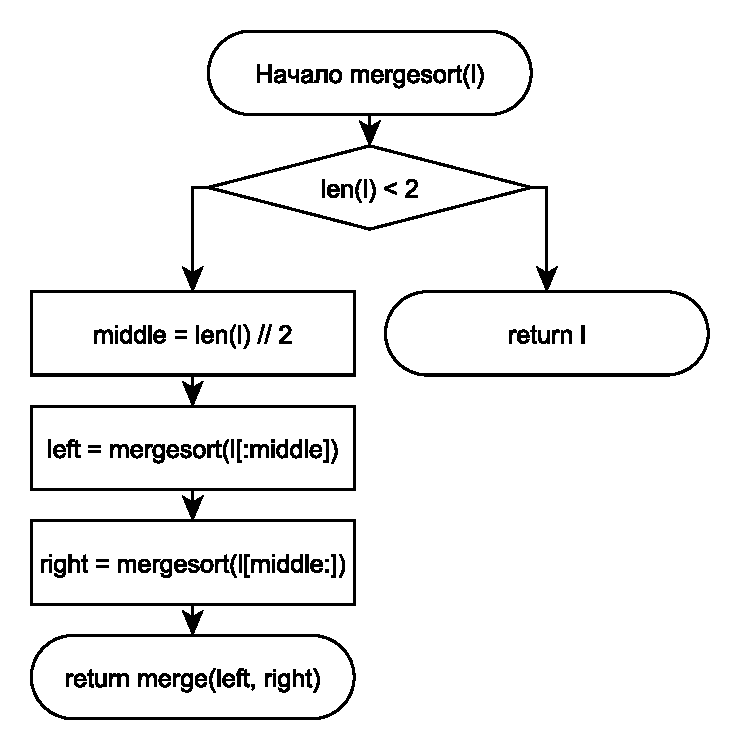
\includegraphics[width=\linewidth]{src/img/1.png}
		\caption{Выбор пути муравьём при отсутствии информации путевых феромонов}
		\label{graph2.1}
	\end{figure}
	
	Допустим, что исходно из каждой вершины вышло по 2 муравья. На рисунке \ref{graph2.2} показано, как распределятся муравьи по путям при отсутствии феромона.
	
	\begin{figure}[H]
		\centering
		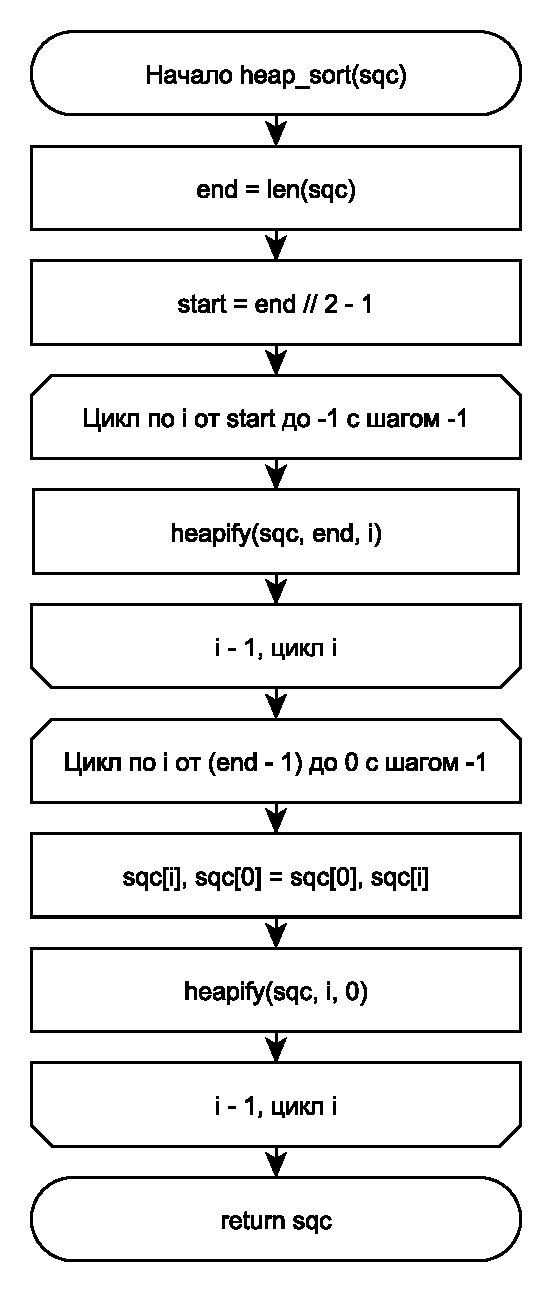
\includegraphics[width=0.7\linewidth]{src/img/2.png}
		\caption{Выбор пути муравьём при отсутствии информации путевых феромонов}
		\label{graph2.2}
	\end{figure}

	Допустим, что все муравьи движутся примерно с одной скоростью. 
	Если дороги были разной длины, то через некоторое время будет оставлено достаточно феромона, чтобы каждый муравей в точке выбора мог однозначно идентифицировать, какой путь был более популярен.
	Таким путём будет более короткий, поскольку муравьи будут проходить его быстрее, следовательно, будет оставлено больше феромона (рисунок \ref{graph2.3}). По мере роста количества феромона у более короткого пути уменьшается количество муравьёв, которые будут выбирать длинную дорогу. 
	
	\begin{figure}[H]
		\centering
		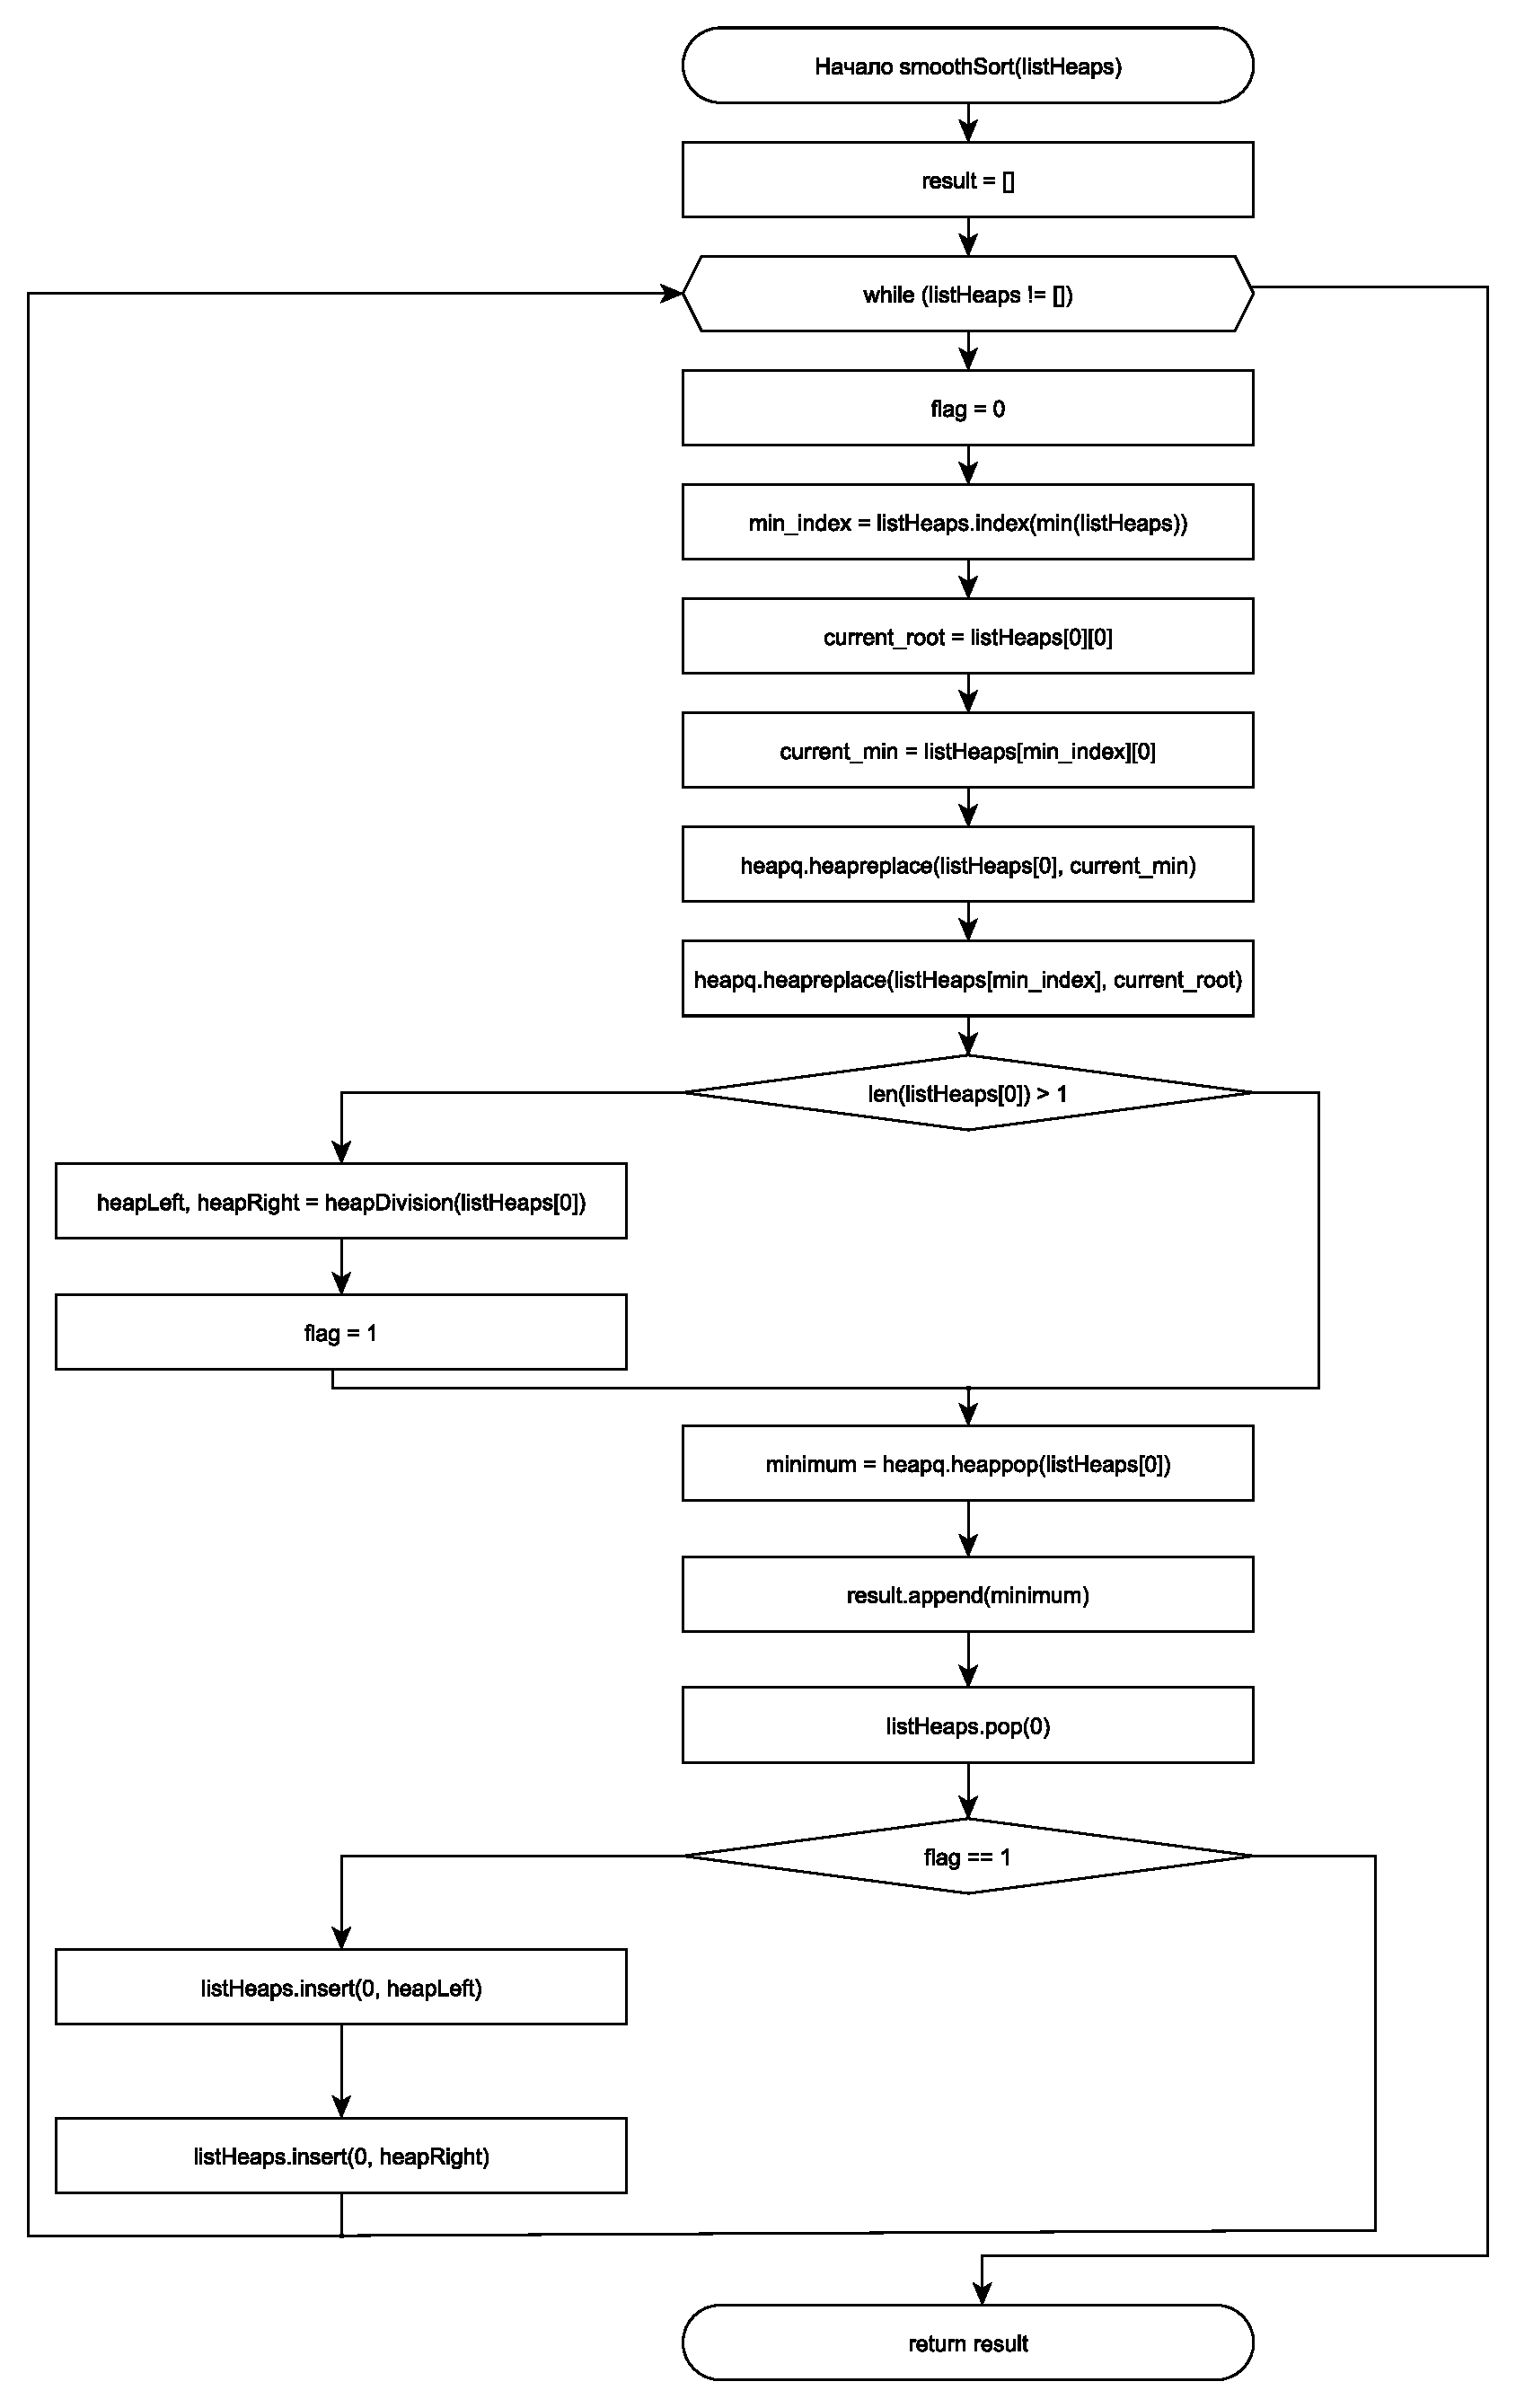
\includegraphics[width=0.7\linewidth]{src/img/3.png}
		\caption{Выбор пути муравьём в результате обработки информации путевых феромонов}
		\label{graph2.3}
	\end{figure}

	Через некоторое время воздействие феромона у длинной дороги будет настолько низким, что все муравьи будут выбирать короткий путь.\cite{ACS}
	
	Для описания поведения муравьёв в реальной жизни введена муравьиная система - алгоритм, в котором искусственно созданные "муравьи" совместно решают проблему обмена информацией через феромон при прохождении вершин графов. Основная идея данного генетического алгоритма состоит в следующем:
	
	\begin{enumerate}[1)]
		\item введём описание данных следующим образом:
		\begin{enumerate}
			\item существуют агенты, "муравьи";
			\item каждый муравей обладает памятью - существует список городов 
			\begin{equation}
				\label{eq2.1} 
				J_{i,k}, 
			\end{equation} 
			которые нужно посетить k-ому муравью, если он находится в городе i;
			
			\item каждый муравей обладает зрением - у муравья есть эвристическое желание посетить город j (находится он при этом в городе i) - это видимость 
			
			\begin{equation}
				\label{eq2.2}
				n_{ij} = \frac {1} {D_{ij}},
			\end{equation}
			
			где D - матрица расстояний (чем короче ребро, тем больше желание пройти по нему);
			
			\item каждый муравей обладает обоняннием - муравей может улавливать феромон, оставленный другими муравьями;
			
			\item происходит непрямой обмен - стигмерж - информацией между муравьями через окружающую среду;
			
			\item муравей использует опыт колонии;
			
			\item у колонии есть время жизни 
			\begin{equation}
				\label{eq2.3}
				1 \leqslant t \leqslant t_{max}
			\end{equation}
			
			\item на каждом шаге по времени все муравьи формируют по маршруту 
			
			\begin{equation}
				\label{eq2.4}
				T_k(t),
			\end{equation}
			
			длины маршрутов
			
			\begin{equation}
				\label{eq2.5}
				L_k(t)
			\end{equation}
			
			можно вычислить;
		
		\end{enumerate}
	
		\item в соответствии с длиной на рёбра маршрута накладывается феромон;
		\item вместе с испарением феромона происходит переход на новый шаг по времени, при этом происходит обновление наилучшего маршрута
		
		\begin{equation}
			\label{eq2.6}
			T^*
		\end{equation}
		
		и длины наилучшего маршрута
		\begin{equation}
			\label{eq2.7}
			L^*
		\end{equation}
		
		в случае, если один из k муравьёв нашёл лучшее решение;
		
		\item если муравей k находится в городе i, то переход в другой город j происходит по вероятностному правилу
		
		\begin{equation}
		\label{eq2.8}
		\begin{matrix}
			P_{ij,k}(t) & = 
			& \left\{
			\begin{matrix}
				0, & \mbox{ } j \notin J_{i,k} \\
				\frac {(τ_{ij}(t))^\alpha * (η_{ij})^\beta} {\sum \limits_{q \in J_{i,k}} (τ_{iq}(t))^\alpha * (η_{iq})^\beta}, & \mbox{ } j \in J_{i,k}, \\
			\end{matrix} \right.
		\end{matrix}
		\end{equation}
		
		где τ - матрица значений феромона, $\alpha$ и $\beta$ - параметры, соблюдающие условие, что $\alpha + \beta = const$;
		
		\item когда маршруты сформированы, каждый муравей оставляет на рёбрах своего маршрута $T_k(t)$ феромон
		
		\begin{equation}\label{eq2.9}
			\begin{matrix}
			\Delta τ_{ij,k}(t) & = 
			& \left\{
				\begin{matrix}
				0, & \mbox{ } (i, j) \notin T_k(t) \\
				\frac {Q} {L_k(t)}, & \mbox{ } (i, j) \in T_k(t), \\
				\end{matrix} \right.
			\end{matrix}
		\end{equation}
		где Q - параметр того же порядка, что и $L^*$ - длина оптимального маршрута;
		
		\item переход на следующий шаг по времени задействует ρ - коэффициент испарения феромона:
		\begin{equation}
			\label{eq2.10}
			τ_{ij}(t+1) = (1-ρ) * τ_{ij}(t) + \sum \limits_{k=1}^m \Delta τ_{ij,k}(t),
		\end{equation}
		где m - размер колонии.
	
	\end{enumerate}
	\cite{RECA}
	
	В начале алгоритма количество феромона принимается равным небольшому положительному числу.
	Общее количество муравьёв остаётся постоянным и равным количеству городов, каждый муравей начинает маршрут из своего города. 
	Данный генетический алгоритм можно модифицировать, введя $e$ элитных муравьёв, которые усиливают рёбра лучшего маршрута $T^*$:
	
	\begin{equation}
		\label{eq2.11}
		\Delta τ_{ij,e}(t) = \frac {e * Q} {L^*}
	\end{equation} \cite{RECA}
	
	
	Сложность алгоритма составляет $O(t_{max} \dot max(m,n^2))$, то есть сложность зависит от времени жизни колонии, количества городов и количества муравьёв в колонии. \cite{RECA}
	
	\begin{algorithm}[H]
		\caption{Муравьиный алгоритм}\label{alg:Ants}
		\begin{algorithmic}[1]
			%\Comment{Под values обобщены непосредственные значения задаваемых параметров; под Parameters, соответсвенно, параметры}
			
			\State $D \gets \_values\_$
			\Comment{Ввод матрицы расстояний}
			
			\State $Parameters \gets \_values\_$
			\Comment{Инициализация параметров алгоритма}
			
			\State $Feromon \gets \_values\_$
			\Comment{Инициализация начальной концентрации феромона}
			\State $η_{ij} \gets \_values\_$
			\Comment{Инициализация видимости}
			
			\State $T^* \gets \_values\_$
			\State $L^* \gets \_values\_$
			\Comment{Выбор начального текущего маршрута и определение длины лучшего текущего маршрута}
			
			\For{t=1;  $t_{max}$; t++}
			\Comment{Цикл по времени жизни колонии}
			\For{k=1; m; k++}
			\Comment{Цикл по всем муравьям}
			\State Построить маршрут $T_k(t)$ по правилу \ref{eq2.8} и рассчитать длину $L_k(t)$.
			\EndFor
			\If { $L_k(t)$ < $L^*$}
			\Comment{Если найден лучший путь}
			\State Обновить $L^*$ и $T^*$
			\EndIf
			\For{рёбра графа}
			\State{Обновить следы феромона на ребре по правилам \ref{eq2.10} и \ref{eq2.11}}
			\EndFor
			\EndFor
			
			\State Print($T^*$ и $L^*$) 
			\Comment{Вывести кратчайший маршрут $T^*$ и его длину $L^*$}
			
		\end{algorithmic}
	\end{algorithm}
	
	В данном разделе поставлена задача. Детально расписаны алгоритмы.
	
\end{document}